\subsubsection{Role Based Access Control} \label{RBAC_SOTA}

\acrfull{rbac}\footnote{\url{https://csrc.nist.gov/projects/role-based-access-control, accessed 01 April 2019}} is a method of controlling access of users in the system, being it physical or online access in the enterprise. It uses policy neutral approach based on roles, where every employee has a role/s assigned, which defines the access levels and resources to be accessed. Mandatory Access Control (MAC) and Discretionary Access Control (DAC) can also be implemented within the system, even though it is different from them. \acrshort{rbac} creates a structure, where firstly the list of privileges (actions, resources, access levels) is defined and assigned to roles. Each role contains a set of privileges and is part of a group where more roles are gathered. Each employee is then assigned a group/s or directly a role/s which authorizes him to access certain resources. This allows more effective management of employees.

The biggest drawback of \acrshort{rbac} is the process of assigning roles and groups being manual, based on request, and not automated. Therefore, when an employee changes a position in a company and new roles is assigned, the previous one should be revoked, but that is often not done and the employee of is granted the access to resources further. Also, it can take a long time before a new role is assigned. On top of that, in case that an employee leaves a company and his access is not revoked, he may still be able to access resources, which is a security threat to a company. Audit of roles and employees’ assignment to them is needed.

\begin{figure}[ht]
    \centering
    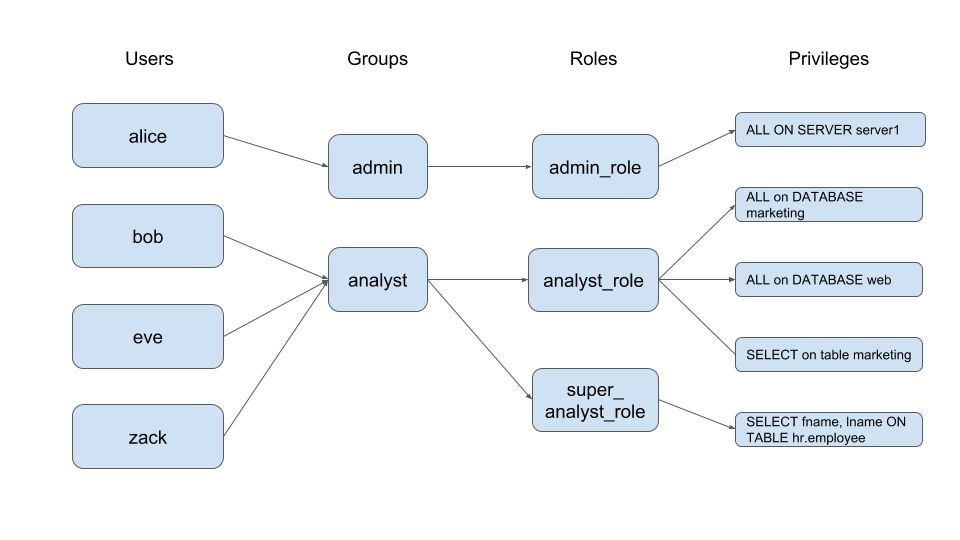
\includegraphics[width=.95\textwidth]{00images/RBAC}
    \caption{Explanation! + new diagram}
    \label{fig:RBAC_diagram_sota}
\end{figure}